\documentclass{article}
\usepackage{graphicx} % Required for inserting images
\usepackage{float} % Required for controlling the position of images

\title{Assignment 2 - DD2424 - Two Layer Network}
\author{Tristan Perrot}
\date{April 2024}


\begin{document}

\maketitle
\begin{center}
    
\includegraphics[scale=0.25]{images/KTH_logo_RGB_svart.png}
\end{center}

\section{Exercise 1}

For this assignment. I decided to create a python object that would represent our classifier. I made this choice because it would simplify the creation of each different classifier and would allow me to easily test different configurations.
\begin{quote}
    \textit{How I checked my analytic gradient computations?}
\end{quote}
After doing the math to compute the gradient and checked it with the given formula on the slides. I decided to implement the gradient computation in the python object. I then compared the results of the analytic gradient with the numerical gradient and the \textbf{PyTorch} gradient.
I use the \textbf{relative error} to compare the gradients for every weights and biases. I get a relative error of $10^{-14}$ for torch vs analytical. However, I get a relative error of $10^{-4}$ for analytical vs numerical and torch vs numerical. The last relative error can be explained because of the numerical approximation of the gradient.

\section{Exercise 2}

\begin{figure}[H]
    \centering
    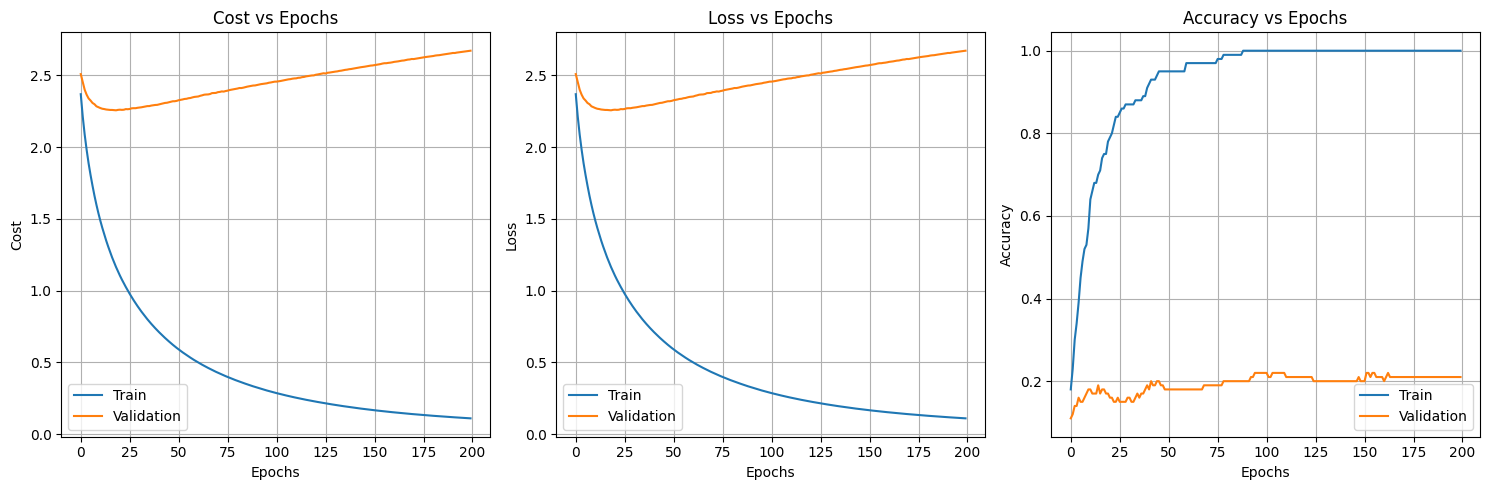
\includegraphics[width=\linewidth]{Result_Pics/ex2.png}
    \caption{Small training with no regularization. It definitely overfits the data.}
    \label{fig:ex2}
\end{figure}

Here, just to see if the classifier works, I trained it on a small dataset with no regularization. As we can see in figure \ref{fig:ex2}, the classifier overfits the data. The training loss goes to zero, but the validation loss increases. This is a clear sign of overfitting. I get these accuracies:
\begin{itemize}
    \item Training accuracy: 100\%
    \item Validation accuracy: 21\%
    \item Test accuracy: 14\%
\end{itemize}

\section{Exercise 3}

\begin{figure}[H]
    \centering
    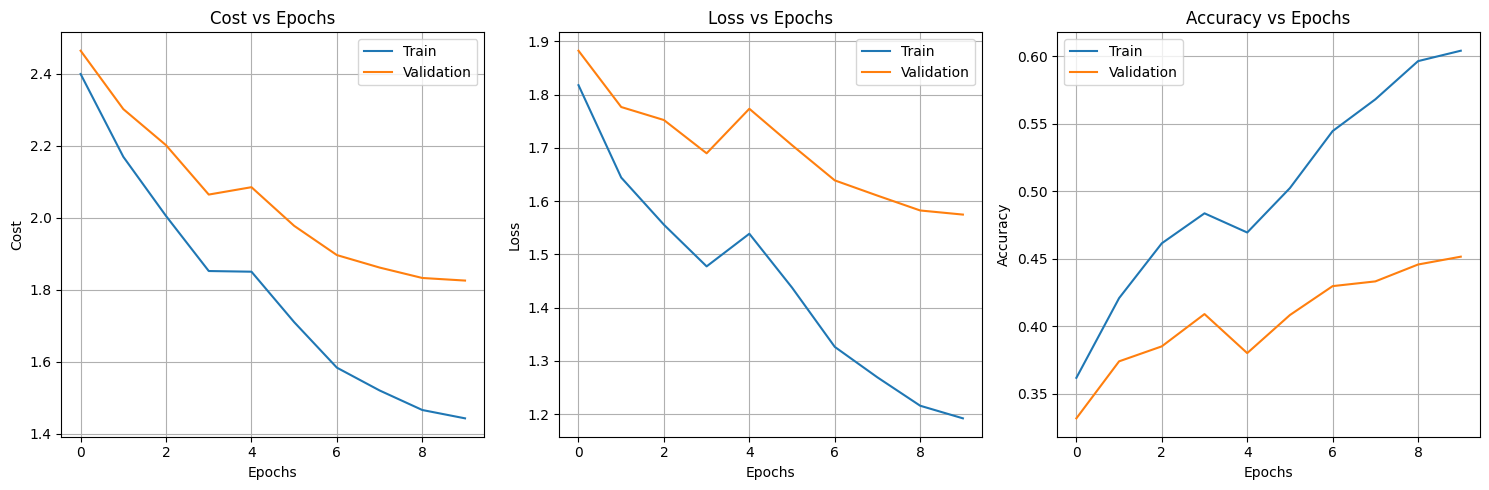
\includegraphics[width=\linewidth]{Result_Pics/ex3.png}
    \caption{\textbf{Training curves (cost, loss, accuracy) for one cycle of training.} The hyper-parameter settings
        of the training algorithm are \texttt{eta min = 1e-5}, \texttt{eta max = 1e-1}, \texttt{lambda = .01}, \texttt{n s = 500} and \texttt{batch size = 100}.}
    \label{fig:ex3}
\end{figure}

Now that the classifier works. I trained the classifier on the CIFAR-10 dataset with cyclical learning rates. Now, the learning rate is not constant but varies between a minimum and a maximum value.

\section{Exercise 4}

\begin{figure}[H]
    \centering
    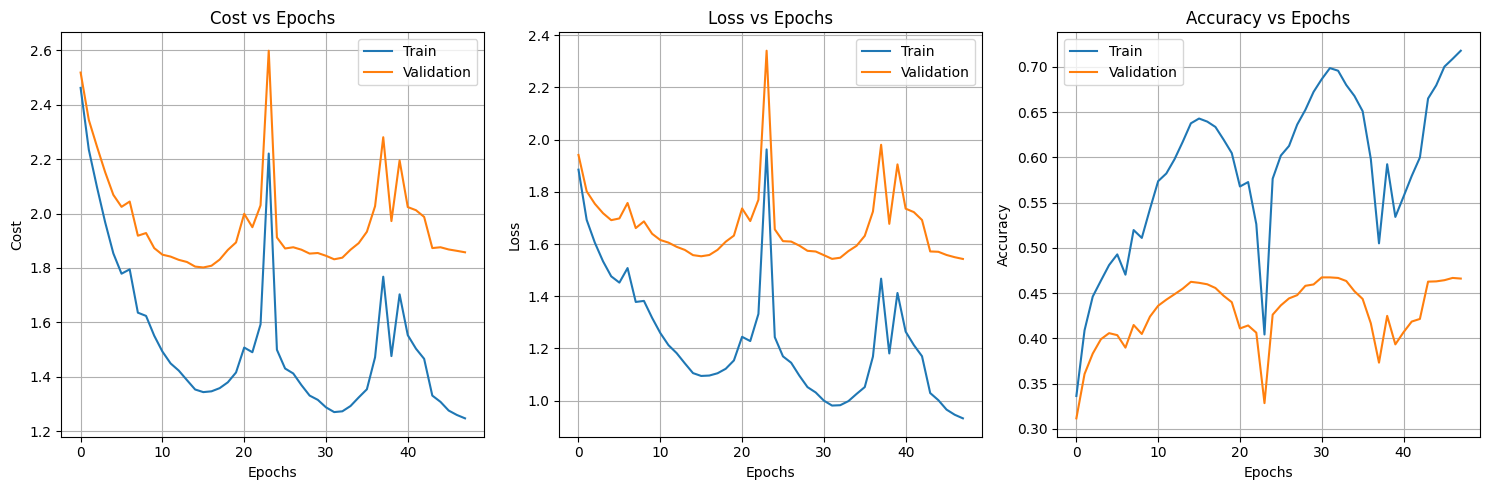
\includegraphics[width=\linewidth]{Result_Pics/ex4.png}
    \caption{\textbf{Training curves (cost, loss, accuracy) for three cycles of training.} The hyper-parameter settings
        of the training algorithm are \texttt{eta min = 1e-5}, \texttt{eta max = 1e-1}, \texttt{lambda = .01}, \texttt{n s = 800} and \texttt{batch size = 100}.}
    \label{fig:ex4}
\end{figure}

Now that the cyclical learning rate works, I trained the classifier on the CIFAR-10 dataset with three cycles of training. As we can see in figure \ref{fig:ex4}, the training loss decreases and the validation loss decreases as well and we can see the cycles. I obtain these accuracies:
\begin{itemize}
    \item Training accuracy: 71.78\%
    \item Validation accuracy: 46.61\%
    \item Test accuracy: 48.09\%
\end{itemize}

\subsection{Coarse to fine lambda search}

\subsubsection{Coarse search}
For the coarse search, I used the \texttt{l min = -5} and \texttt{l max = -1} (so with \texttt{lambda} between \texttt{$10^{-l min}$} and \texttt{$10^{-l max}$}) and I used 20 values between these two values randomly chosen. I trained the classifier for 2 cycles. I obtain this top 3 results:
\begin{itemize}
    \item Lambda: 8.887e-05, Accuracy: 47.3\%
    \item Lambda: 0.0007362, Accuracy: 46.8\%
    \item Lambda: 0.0008308, Accuracy: 46.4\%
\end{itemize}

\subsubsection{Fine search}
For the fine search, I used the worst lambda and the best lambda from the top 5 results of the coarse search. I used 20 values between these two values randomly chosen. I trained the classifier for 2 cycles. I obtain this top 3 results:
\begin{itemize}
    \item Lambda: 0.0001349, Accuracy: 47.1\%
    \item Lambda: 4.93e-05, Accuracy: 45.7\%
    \item Lambda: 0.0001497, Accuracy: 45.7\%
\end{itemize}

\subsection{Final test accuracy}
After that I have redone a fine search with the same method as before but with the best lambdas from the fine search. I obtain the best lambda: 0.0003 with an accuracy of 48.5\% on the validation set.
Then, with this parameter, a \texttt{n s = 600}, 5 cycles of training and a batch size of 200.

\begin{figure}[H]
    \centering
    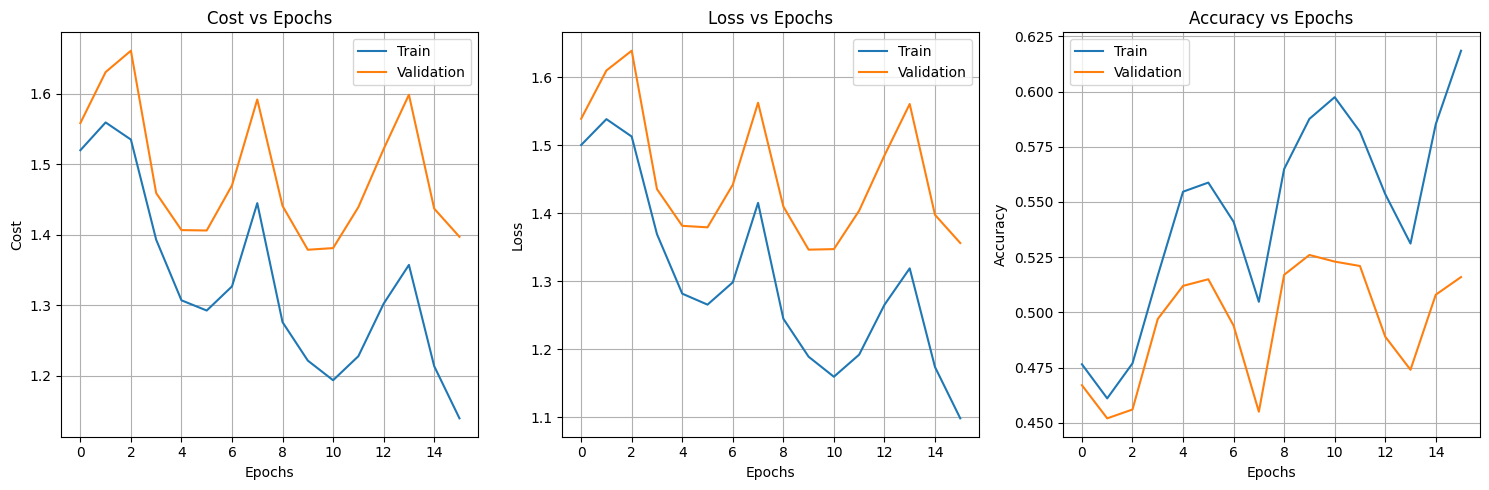
\includegraphics[width=\linewidth]{Result_Pics/final-perf.png}
    \caption{\textbf{Training curves (cost, loss, accuracy) for eight cycles of training.} After the coarse and fine search.}
    \label{fig:final}
\end{figure}

I obtain these accuracies:
\begin{itemize}
    \item Train Accuracy: 63.12\%
    \item Validation Accuracy: 52.2\%
    \item Test Accuracy: 51.49\%
\end{itemize}

\section{Conclusion}
In conclusion, I have implemented a two layer neural network with a cyclical learning rate and a regularization term. I have trained this classifier on the CIFAR-10 dataset and I have done a coarse and fine search for the regularization term. I have obtained a test accuracy of 51.49\% which is not bad for a two layer neural network.

\end{document}